\epigraph{\textit{""}}

\paragraph{Abstract} Characterization of perovskite solar cells is a non-trivial subject, the techniques researchers successfully employed for \gls{osc} and \gls{dssc} needs to be re-validated for this new kind of solar cells.
The presence of ionic migration in the absorber can be a game-changer for which special care has to be taken.

\section{Conventions and General Remarks}

	All the characterization on complete devices was performed keeping them in an air-tight holder filled with nitrogen.
	The electrical connection from the cell electrode to the external end of the holder was obtained using gold tips connected via a printed circuit board to a coaxial cable.

	\subsection{Sign Convention and Parameters Definitions}

		\paragraph{Fermi level} The electrons electrochemical potential, also known as Fermi level, is defined as the energy required for adding an electron in a specified position.
		Its value depends on the electrostatic potential $V$ in that position and on the internal chemical potential $\mu$ which in our case depends mainly on the concentration of electrons (not related to their electric charge, similarly to the density of a gas).
		As the Fermi level is going to be used mainly for comparisons, its zero is not going to be defined thesis-wide, instead it will be defined to a convenient reference just where needed.

		\paragraph{Cathode and anode} Considering a solar cell device at steady state under illumination and in open circuit conditions, its cathode is defined as the contact where the electrons electrochemical potential $\bar\mu$  is the highest.
		By consequence the other contact is the anode.
		The naming of the two contacts holds to the one defined in illuminated, open circuit conditions even in conditions where the contacts' electrochemical potential is in the reversed order.

		\paragraph{Voltage} The voltage $\Delta V$ is always used as a relative value, defined subtracting the electrons electrochemical potential of the cathode from the anode's one.
		So in the aforementioned solar cell example, the voltage is positive.
		The unit is the Volt.

		\paragraph{Electrical power} The electrical power $P$ is defined as positive when the device absorbs electrical energy (incoming, passive element) and negative when it generates energy (outgoing, active element).
		It can be expressed in extensive form with power (Watt) unit or in intensive form "electrical power density" with power over active area unit (Watt over square centimetre).

		\paragraph{Current} The current $J=P/V$ is measured through an external circuit and the sign is a consequence of the voltage and electrical power definition: A current ("conventional current", flow of positively charged particles) being released from the device's anode and being received from the device's cathode is defined as negative.
		This can be thought as: Inside the device, somehow, a positive charge was moved from the high Fermi level contact to the low Fermi level contact, increasing its electrochemical energy, the opposite to what would happen in a resistor, whose current is always positive.
		In a solar cell device, the current and the electrical power can be either positive or negative depending on the illumination and voltage conditions.
		It can be expressed in extensive form with current (Amperes) unit or in intensive form "current density" with current (Amperes) per active area (square centimetre) unit.

		\begin{SCfigure}
			\centering
			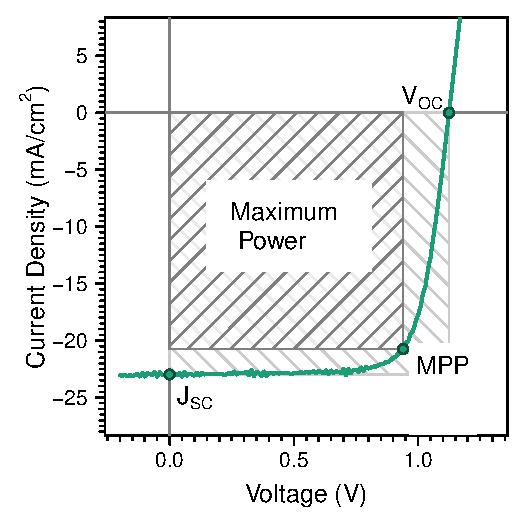
\includegraphics[width=0.5\textwidth]{iv_params/IV-revIVs.pdf}
			\mycaption[Parameters extraction from current-voltage sweeps.]{A typical current-voltage sweep is represented.
				MPP stands for maximum power point, \gls{jsc} stands for \glsdesc{jsc}, \gls{voc} stands for \glsdesc{voc}.
				The ration between the small and the large rectangles areas is the \glsdesc{ff} (\gls{ff}).}\label{fig:iv_params}
		\end{SCfigure}

		\paragraph{\Glsdesc{voc}} \Gls{voc} parameter is defined as the voltage $\Delta V$ at which the current is zero while the solar cell device is illuminated at 1~sun conditions and in steady state (positive by its own definition).

		\paragraph{\Glsdesc{jsc}} \Gls{jsc} parameter is defined as the unsigned value of the current density flowing in an external circuit short circuiting (zero resistance) the solar cell device's contacts while illuminated at 1~sun and in steady state.
		It is usually reported in current (milli Amperes) over active area (square centimetre) unit.

		\paragraph{Maximum power density} The maximum power density is defined as the unsigned minimum of electrical power density which can be obtained by $P(V) = J(V) \cdot V$.
		It is usually reported using power (Watt) over active area (square centimetre) unit.

		\paragraph{\Glsdesc{pce}} \Gls{pce} parameter is defined as the maximum power density over the illuminating power density, which at 1~sun AM 1.5G is defined to \SI{100}{\mW\per\square\cm}.
		It is usually reported as a percentage.

		\paragraph{\Glsdesc{ff}} \Gls{ff} parameter is defined as the ratio between \gls{pce} and the product of \gls{voc} and \gls{jsc}.
		This parameter does not have a physical meaning, but it represents how much the series and shunt resistances affect the device efficiency.

		\paragraph{Forward and reverse bias} Forward bias is a device condition where the voltage is positive, reverse bias is the case where the voltage is negative.

		\paragraph{Forward and reverse scan} In current-voltage sweeps, a scan where the voltage is increasing over time is a forward scan, while a voltage variation in the opposite direction constitutes a reverse scan.

		\paragraph{Ideality factor} An ideality factor $n_{id}$ different from 1 describes deviations from the ideal photo-diode.
		The adapted $J(V,\phi)$ equation becomes\cite{Calado2018b}:
		\begin{equation} \label{eq:photodiode}
			J = J_{SC}(\phi) - J_0\left(\exp\left(\frac{qV}{n_{id}k_BT}\right)-1\right)
		\end{equation}
		where $J_0$ is the diode saturation current (the current flowing in dark when applying a reverse bias), $q$ is the elementary charge, $k_B$ is the Boltzmann constant, and $T$ is the temperature.
		Clearly the reported equation just offers a simplified model.
		For example, it can be improved adding the contribution from the series resistance $R_s$ and would become

		$$J = J_{ph}(\phi) - J_0\left(\exp\left(\frac{q(V+JR_s)}{n_{id}k_BT}\right)-1\right)$$

		where now $J_{ph}$ is the total photo-generated current.
		The function is now an implicit one, requiring numerical solving even for obtaining $J_{SC}$.

		\paragraph{Top and bottom of devices} The point of view of the manufacturer is used for defining the physical top and bottom of a device: the bottom is the glass substrate and the top is the last deposited layer.
		This is opposite with the usage of a solar cell in the real world and with most of the solar simulators (but not all of them, for example Paios from Fluxim has an illumination from below, more convenient for contacting the electrodes without a samples holder \cite{Fluxim}).

	\subsection{Usage of Shadowing Mask}

		\begin{SCfigure}
			\centering
			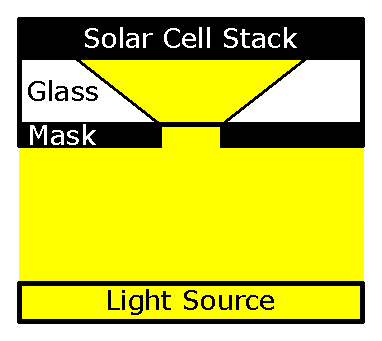
\includegraphics[width=0.5\textwidth]{shadowing_mask/shadowing_mask.pdf}
			\mycaption[Illuminated area after a shadowing mask.]{This schema is just for explaining the concept described in the text, its dimensions are not realistic.}\label{fig:shadowing_mask}
		\end{SCfigure}

		In literature is generally suggested to use a shadowing mask when measuring the solar cell devices in order to better define the illuminated area (as in the broken \cite{Brinser2017} form from Nature\cite{NatureResearch2017}).
		%, the file is a dynamic XFA form and cannot be opened by most PDF readers (and they rightly do not, as it was deprecated in ISO 32000-2:2017), Adobe products or Master PDF Editor is required for reading).
		In our case the active area is just \SI{0.09}{\square\cm} so the mask aperture should be extremely small and its exact positioning troublesome.
		Additionally, the fact that the illumination reaches the mask from a wide angle (the illuminating source dimension, which is not just the lamp as the illumination passes through spread lenses, is not small compared to the lamp-cell distance) allows the light to spread through the substrate glass (\SI{2.2}{\mm} for \gls{fto} substrates, other groups use even thicker glass substrates) reaching a significantly larger area on the active layer at the other side of the glass, as represented in \cref{fig:shadowing_mask}.
		In our solar simulator a linear widening of 8~\% over \SI{2}{\mm} was estimated, this makes an illuminated area 16~\% larger than the mask aperture.
		Even if the total incident power is still determined from the mask aperture, the illumination intensity is not 1~sun any more, compromising the validity of a measurement done with a shadowing mask.


	\subsection{Stability During the Measurement and Small/Large Perturbations}

		Most of the reported hybrid lead halide perovskite materials can show rather impressive changes in their structure on long time scales, for example due to ionic migration \cite{Calado2016}, degradation \cite{OKane2019}, and self-healing \cite{Ceratti2018}.
		This have to be taken into account for all the measurements techniques output which either takes too long time to be measured or employs large perturbations.

		\paragraph{Long lasting measurement} An example of the first case is the impedance spectroscopy where during the long lasting measurement various phenomena can occur, like: a slow current evolution due to perovskite well known hysteretic behaviour prior to stabilization; a degradation process changing the current; the heating of the device changing its properties.
		This slow current evolution can easily be misinterpreted for capacitive current \cite{Jacobs2018} and introduce artefacts like loops in the Nyquist plots \cite{Moia2019}.

		\paragraph{Large perturbations} \label{perturbation}
		Large perturbations regime means that the independent variable being perturbed is changed by an amount large enough to cause the quantity under study to not follow the approximation given by the first term of its series expansion.
		Let's take some example.

		\paragraph{Large perturbations -- \gls{tpv}}
		For example, if too intense, the light pulse in \acr{tpv} could change the voltage by a less-than-linear amount.
		In this case, the light pulse is not only probing the recombination, but it is adding some, so a large perturbation has to be avoided.
		This effect has been reported for \gls{dssc} in \authoryear{Barnes2013}.

		\paragraph{Large perturbations -- impedance}
		Another example: a too wide sinusoidal voltage oscillation amplitude in impedance measurements can cause a non-sinusoidal current output.
		This is not a problem for the measurement itself, as the lock-in amplifiers are perfectly able to extract the amplitude and the phase of the signal first harmonic, ignoring the higher harmonics caused by the too large perturbation.
		But artefacts could arise and cause misinterpretations, as explained in \cpageref{impedance-large_perturbations}.

		\paragraph{Large perturbations -- \gls{trpl}}
		Last example: in the \glsdesc{trpl} a laser pulse illuminates the otherwise unilluminated absorber layer.
		This pulse induces a the migration of the ionic defects to a new profile depending on the pulse intensity \cite{Levine2018}, by a small extent due to its short duration.
		The fact that the relaxation time of the ionic migration is usually much larger than the laser repetition rate (\si{\ms} to seconds for the ions \cite{Jacobs2018} and \si{\ms} to \si{\us} for typical \gls{trpl} lasers \cite{EdinburghInstruments}) implies that the ionic profile variation slowly "builds up" pulse after pulse.
		As the ionic profile affects the free charges concentration, and this in turn rules the radiative recombination, the measurements of \gls{trpl} have to be done with extreme care.
		An example of hysteretic behaviour observed with \gls{trpl} can be found in \authoryear{Motti2016} and elsewhere \cite{Chen2015,Chen2017}.
		This should also be considered when comparing life-times from different laser fluences \cite{Manser2014}.

\section{Current-Voltage Sweeps}

	After calibrating the light intensity in the solar simulator (see \cpageref{solarsimulator}), the devices were exposed to the illumination at open circuit for some seconds in order to have a stabilized open circuit voltage.
	Then usually the curves were measured with the auto-measure function of the PyPV software (see \cpageref{automeasure}) which measures the reverse scan and then the forward scan.

	\paragraph{Parameters Extraction from Sweeps}
	For the devices studied in this thesis, the reported values of \gls{voc}, \gls{jsc}, \gls{pce} and \gls{ff} are extracted from a forward or reverse current-voltage sweep.
	This is in accordion to the tradition of solar cells reporting but for hysteretic devices, like perovskite solar cells, a static measurement should be preferred.
	%Checking the aforementioned definitions, one can easily notice how this is not the correct way as these parameters need to be measured in steady-state conditions.
	%This is comes from the tradition of solar cell reporting, which was established in pre-hysteresis times and is no longer a valid approximation.
	%Apologizing for the lack of coherence I hope I'll be able to implement the static measurements of \gls{voc} and \gls{jsc} in the PyPV measurement routines (described in \cpageref{automeasure}).

	\paragraph{Parameters Extraction from Sweeps -- \gls{pce}} Regarding the \gls{pce}, and by consequence the \gls{ff}, a proper measurement is made difficult due to the cell evolution over time (hysteresis).
	The voltage associated to the maximum power point is drifting and its localization affects its evolution.
	A proper \gls{mppt} system needs to be bought or developed, see \cpageref{software_mppt} for thoughts about possible implementations.

	\paragraph{Auto-scale}\label{autoscale} In literature one can easily find current-voltage curves with discontinuities or "kinks" \cite{Li2016,Snaith2014,Zhang2015} like the one reported in \cref{fig:autoscale}.
	Some even lucubrate about the origin of these in perovskite solar cells.
	Indeed this is likely just caused by the auto-scale feature of the Keithley equipment, disabling this, the discontinuities disappears.

	\begin{SCfigure}%[!hbtp]%
		\centering
		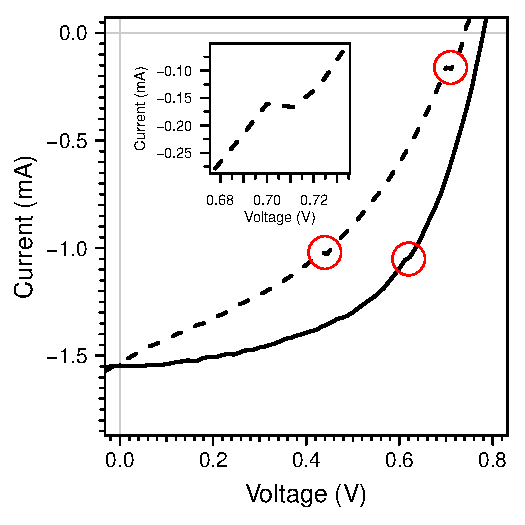
\includegraphics[width=0.5\textwidth]{autoscale/ig1-3-1-int4.pdf}
		\mycaption[Kinks in JV sweep due to autoscale.]{A current-voltage sweep of an hysteretic perovskite solar cell with Keithley autoscale active.
			Both the forward (dashed) and the reverse (solid line) present small discontinuities around \SI{1}{\mA} and \SI{0.1}{\mA}.}\label{fig:autoscale}
	\end{SCfigure}

	\paragraph{Scan speed} The used sweep speed is \SI{500}{\mV\per\s}, which was arbitrarily chosen for avoiding bumps leading to currents higher than \gls{jsc}, like the one in \cref{fig:iv_ugly} (seldom reported in literature, like in figure~S3 of \cite{Du2018} and simulated with drift-diffusion in \cite{Walter2018}).
	%having an aesthetically good looking current-voltage curve
	Our arbitrary choice allowed us to make fair comparisons between devices, but the absolute values should be considered as approximations.
	\begin{SCfigure}%[!hbtp]%
		\centering
		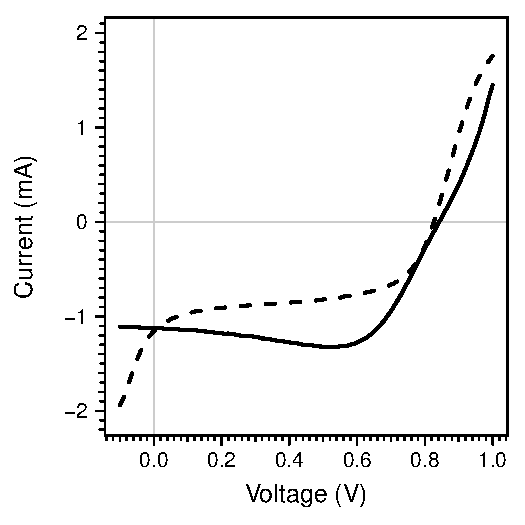
\includegraphics[width=0.5\textwidth]{iv_ugly/ig47-b32-int2-4.pdf}
		\mycaption[Hysteretic current-voltage scan.]{At the employed scan speed, the hysteresis phenomena causes the reverse (solid line) scan to reach currents higher than the \gls{jsc}.}\label{fig:iv_ugly}
	\end{SCfigure}
	We wanted to underline that due to hysteresis phenomena, no scan speed, direction, or precondition is the correct one.
	% and they all heavily affect the resulting \gls{pce}.
	Rather, a static measurement or a \acr{mppt} should be used for obtaining a accurate and realistic result.
	This comment regards also the so-called "hysteresis-free" perovskite solar cells, which can also have hysteretic phenomena\cite{Jacobs2018,Du2018}.

	\paragraph{Noise} The noise often observed in current-voltage sweeps at high scan speeds in this thesis is mainly caused by oscillations in the solar simulator illumination intensity, as an example see \cref{fig:iv_params}.
	For reducing the noise impact on the \gls{jsc} and \gls{voc} parameters extraction, these values were extracted via a parabolic fitting.
	%Indeed, using a white \gls{led} as illumination source, this noise is not present but the spectral mismatch affects the meaningfulness of the measurement.

	\paragraph{Stabilized or dynamic current-voltage sweeps} One very appealing alternative to current-voltage sweeps are the so-called "stabilized current-voltage sweeps", where at each voltage point a fixed stabilization time is waited and the stabilised current is reported \cite{Unger2014, Christoforo2015}.
	An improvement of this technique is named "dynamic current-voltage sweeps", here the stabilization step is of variable duration, until the current-time derivative falls below a threshold (\textit{e.g.}\ \SI{0.2}{\%\per\minute}) \cite{Dunbar2017,Dunbar2017a}.
	In this thesis, these techniques have not been used.

	\paragraph{Shunt and series resistances} \label{resistances} In our group the shunt and series resistances are evaluated by the current \textit{versus} voltage derivative of a dark current-voltage sweep respectively at zero and at high-enough voltage.
	This methodology is inherited from organic solar cells and, as is easy to foresee, is unreliable on hysteretic devices: in the case of perovskite solar cells a measurement of the stabilised current at a few points have better chances to produce a useful result.
	The measurement of the current at a voltage close to zero is enough for estimating the shunt resistance while two points at high voltages are needed for estimating the series resistance.

\section{V\textsubscript{OC} and J\textsubscript{SC} Dependence on Light Intensity}
	The solar simulator illumination intensity $\phi$ is reduced via neutral density filters with transmittance of 0.05, 0.12, 0.25, 0.51, 0.81 and 1 (no filter).
	The values of $V_{OC}(\phi)$ and $J_{SC}(\phi)$ can be obtained from static measurements or from current-voltage sweeps.
	The static measurement of $V_{OC}(\phi)$ at high light intensities is troublesome as it can easily damage the device.
	In this thesis, the used method is specified case by case.
	%this measurement is reported both from static measurement of \gls{voc} and from \gls{voc} obtained from current-voltage sweeps; the used method is specified case by case.
	%The devices are kept at this reduced illumination $\phi$ and at open circuit or short circuit conditions until steady state for measuring respectively 

	\subsection{\Gls{jsc} \textit{versus} $\phi$}
		The \gls{jsc} dependency on the light intensity $\phi$ is close to linear and can be fitted with a power law:
		\begin{equation} \label{eq:jsc-phi}
			J_{SC} \propto \phi^\alpha
		\end{equation}
		giving $\alpha$ values usually from 0.95 to 1.

		\paragraph{Interpretation} %The \gls{jsc} dependency on the light intensity $\phi$ is close to linear and can be fitted with a power law $J_{SC} \propto \phi^\alpha$ as described in \cpageref{methods_jsc_intensity}.
		An $\alpha$ value lower than 1 indicates the presence of non-geminate recombination (for geminate recombination see \cpageref{intro_geminate}) at short circuit\cite{Credgington2011}, indicating that not all the photo-generated charges get extracted, neither at short circuit conditions.

	\subsection{\Gls{voc} \textit{versus} $\phi$ and the Ideality Factor $m$}
		Setting $J=0$, which corresponds to open circuit conditions, in \cref{eq:photodiode} (without considering the series resistance correction) we can obtain a relation between \gls{jsc} and \gls{voc}:
		%\begin{equation} \label{eq:photodiode-zerocurrent}
		$$J_{SC}(\phi) = J_0\left(\exp\left(\frac{qV_{OC}(\phi)}{n_{id}k_BT}\right)-1\right)$$
		%\end{equation}
		This equation can already be used for obtaining the $n_{id}$ and $J_0$ values fitting the \gls{jsc} and \gls{voc} measured at different light intensities $\phi$ (also varying the temperature could be used for fitting the values, but it was not done during this thesis).

		Solving for \gls{voc} we obtain:
		%\begin{equation} \label{eq:photodiode-zerocurrent-voc}
		$$V_{OC} = \frac{n_{id}k_BT}{q}\cdot\ln\left(\frac{J_{SC}}{J_0} + 1\right)$$
		%\end{equation}

		Considering that the saturation current $J_0$ (current in dark under reverse bias) is much smaller than $J_{SC}$ for the light intensities we usually employ (down to \SI{0.05}{suns}), we can approximate to:
		%\begin{equation} \label{eq:photodiode-zerocurrent-voc_approx}
		$$V_{OC} \approx u_1 + \frac{n_{id}k_BT}{q}\cdot\ln(J_{SC})$$
		%\end{equation}

		where $u_1$ is a useless constant.
		Then if the $\alpha$ value is close enough to~1, we can use \cref{eq:jsc-phi} and further approximate for plotting against light intensity $\phi$:
		\begin{equation}\label{eq:voc_vs_phi}
			V_{OC}(\phi) \approx u_2 + \frac{n_{id}k_BT}{q}\cdot\ln(\phi)
		\end{equation}

		This is the equation we commonly employ for fitting and obtaining ideality factors \cite{Nelson2003}.
		In some cases this latest expression is used as ideality factor definition as it conveniently uses a zero current measurement (\gls{voc}) so that series resistance can be completely ignored \cite{Kirchartz2012}.
		%In literature one can found reports of ideality factor determined via \gls{voc} versus \gls{jsc} dependency. The results of the latter method may differ from the aforementioned one due to series resistance and the non-linear dependency of the \gls{jsc} from the light intensity ($\alpha < 1$). 
		The so-obtained ideality factor $n_{id}$ is usually from 1 to 2.
		A voltage dependent ideality factor can also be measured from a current-voltage sweeps in dark but has not been evaluated in this thesis, as it would be affected by hysteresis.
		A critical analysis of these methods and the proposal of a new "Transient Suns-\gls{voc}" method (employing a pre-biassing for flattening the ionic profile) can be found in \authoryear{Calado2018b}.
		% Anyway in perovskite solar cells exhibiting hysteresis, a current-voltage sweep would not give fair ideality factors and the current-voltage points should be acquired reaching steady state conditions for each point. Both these methods for deriving the ideality factor have been implemented in the DrIFtFUSION simulation as described in \cpageref{dd_ideality}.

		\paragraph{Interpretation} %\The \gls{voc} dependency on the light intensity $\phi$ can be fitted with a natural logarithmic dependence obtaining the ideality factor $m$. 
		\authoryear{Pockett2015} measured ideality factors of planar perovskite solar cells via stabilized \gls{voc} obtaining, for some cases, values as high as 5.
		Also in organic \cite{Kirchartz2011,Kirchartz2012} and silicon solar cells \cite{Breitenstein2006} ideality factors greater than 2 has been observed and explained.
		According to \authoryear{Calado2018b} and \authoryear{Kirchartz2012}, the ideality factor, once obtained in the correct way, is 1 when studying most of the recombination types and 2 for mid-gap trap mediated recombination in regions where the electrons and holes concentrations are similar, $n \approx p$.

\section{Charge Extraction (CE)}

	\paragraph{Concept} The charge extraction experiment has been designed\cite{Duffy2000} to quantify the free charges available in a device.
	After stabilization of a device at a light intensity and an applied voltage (in our case always at \gls{voc}), the illumination is switched off and the electrodes of the device are short circuited.
	The transient current flowing through the short circuiting circuit can be measured and integrated to estimate the available charge.
	The integrated charge has to be considered as a lower bound to the actually present excess charge, as part of it could recombine inside the device during the extraction time \cite{ORegan2005}.
	%\paragraph{Limitations -- from \gls{osc}}

	\paragraph{Limitations specific of perovskite solar cells} \label{ce_limitations_perovskite}When measuring the \gls{ce} of a perovsktie solar cell, additionally to the aforementioned limitations, one should also consider that the ionic profile update (from $V=V_{OC}$ to $V=0$) causes a displacement current, as described in \cpageref{intro_displacement_current}.
	A simulation with DrIFtFUSION is reported for an homojunction device in \cref{fig:ce_single_dd}, it can be seen that with ionic mobile defects in \cref{fig:ce_single_dd-ions_zoom} a very weak but long lasting current appears and gives a relevant contribution to the integrated charge.
	This will happen on very large time scales and it will not affect the short measurements used for the free charges estimation, so it is rarely reported\cite{ORegan2015b}.
	The charge measured in the external circuit due to the ionic displacement current could be underestimated as the free charges rearrangements can also occur through the perovskite layer rather than through the external circuit.

	\begin{figure}
		\makebox[\textwidth][c]{
			\parbox{1.1\textwidth}{
				\centering
				\begin{subfigure}[t]{0.5\textwidth}
					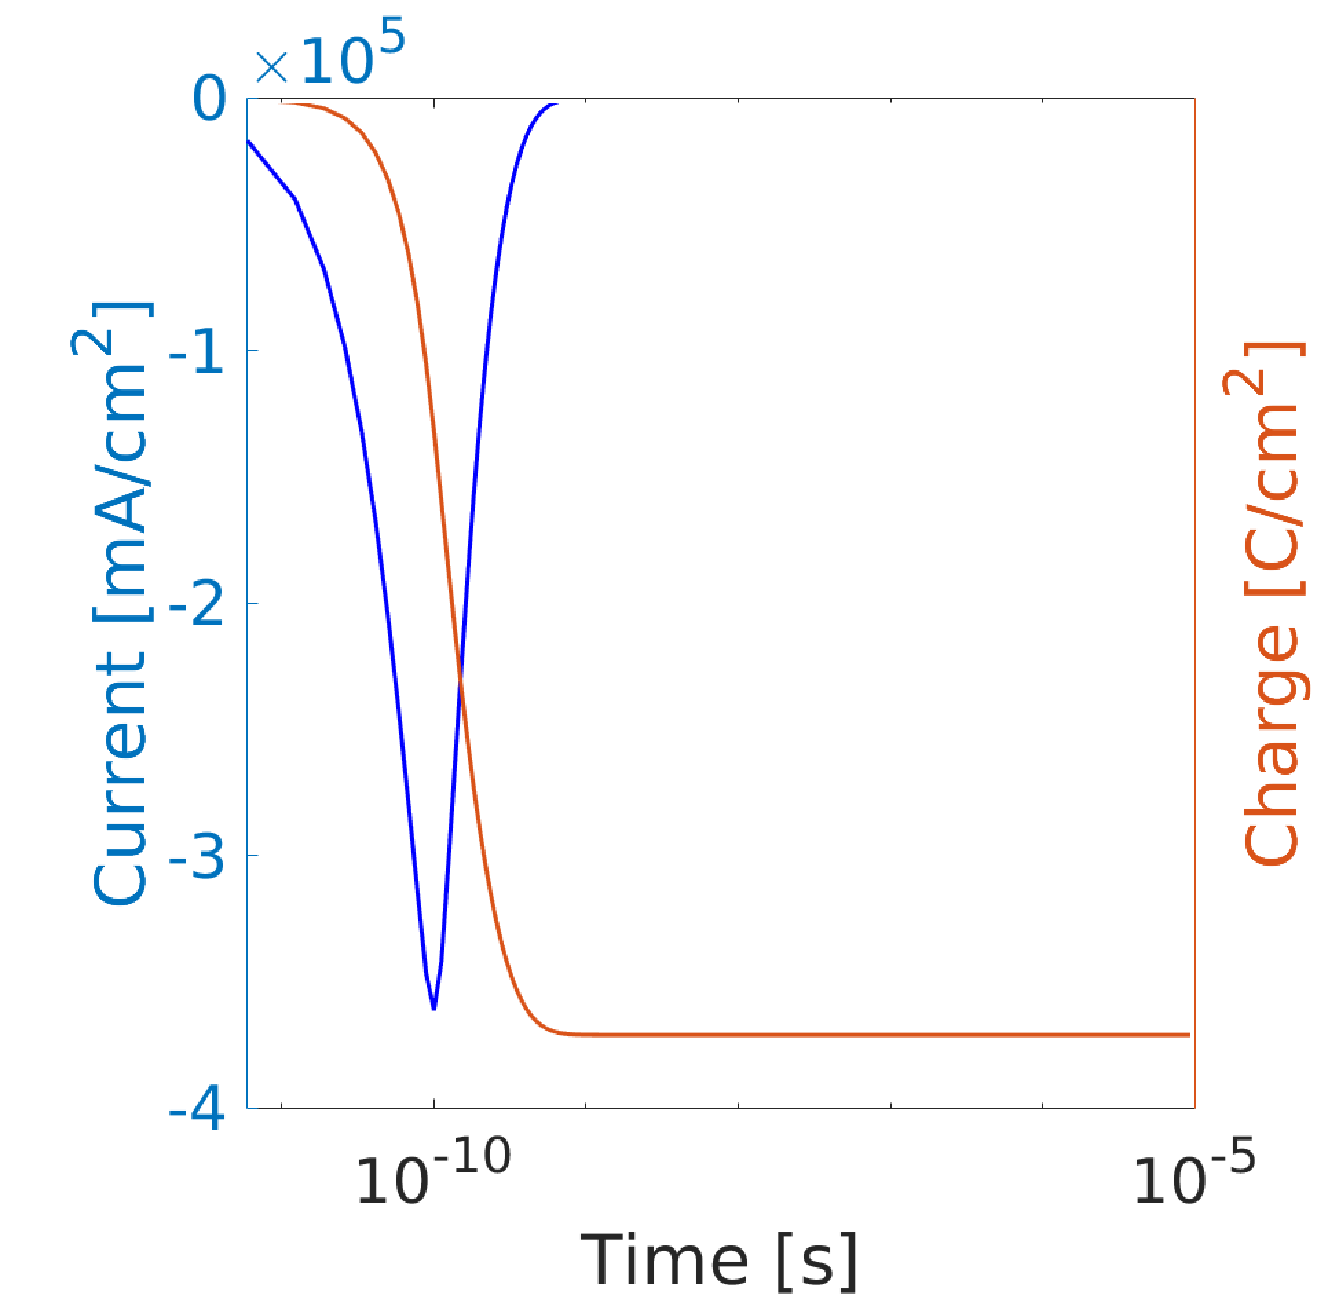
\includegraphics[width=1\textwidth]{ce_single_dd/ce_single_dd-noions.pdf}
					\subcaption{Without mobile ions}\label{fig:ce_single_dd-noions}
				\end{subfigure}
				\bigskip

				\begin{subfigure}[t]{0.5\textwidth}
					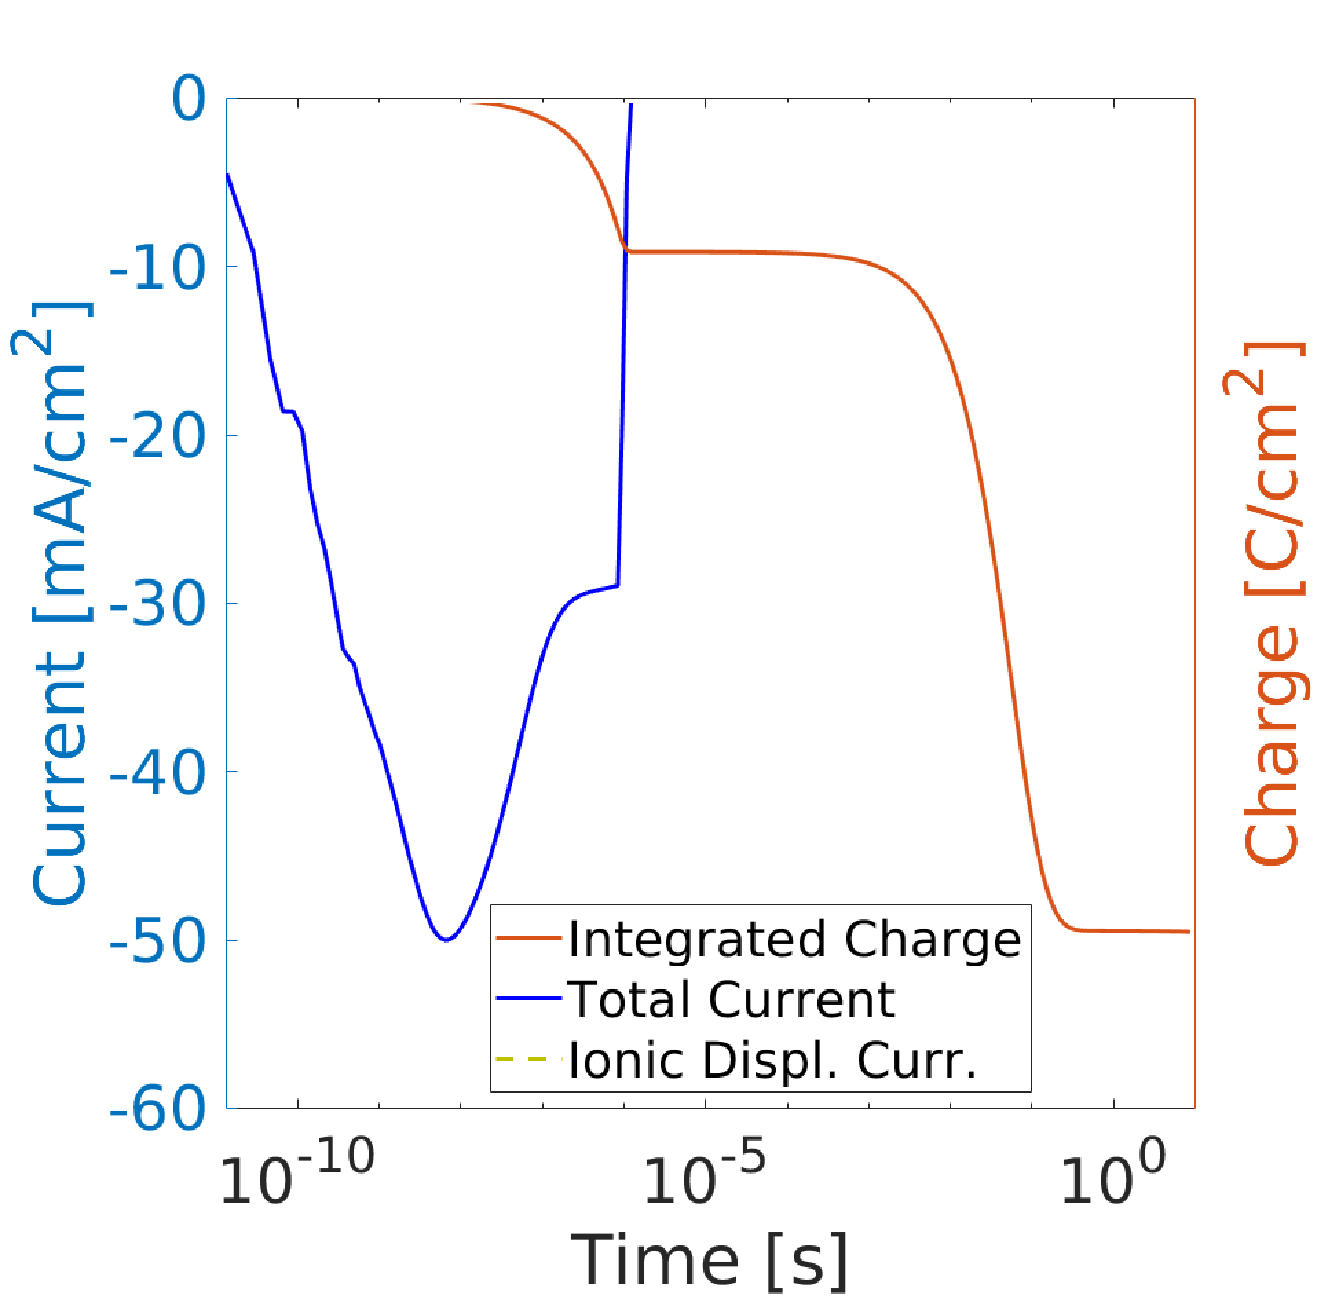
\includegraphics[width=1\textwidth]{ce_single_dd/ce_single_dd-ions.pdf}
					\subcaption{With mobile ions}\label{fig:ce_single_dd-ions}
				\end{subfigure}
				\qquad
				\begin{subfigure}[t]{0.5\textwidth}
					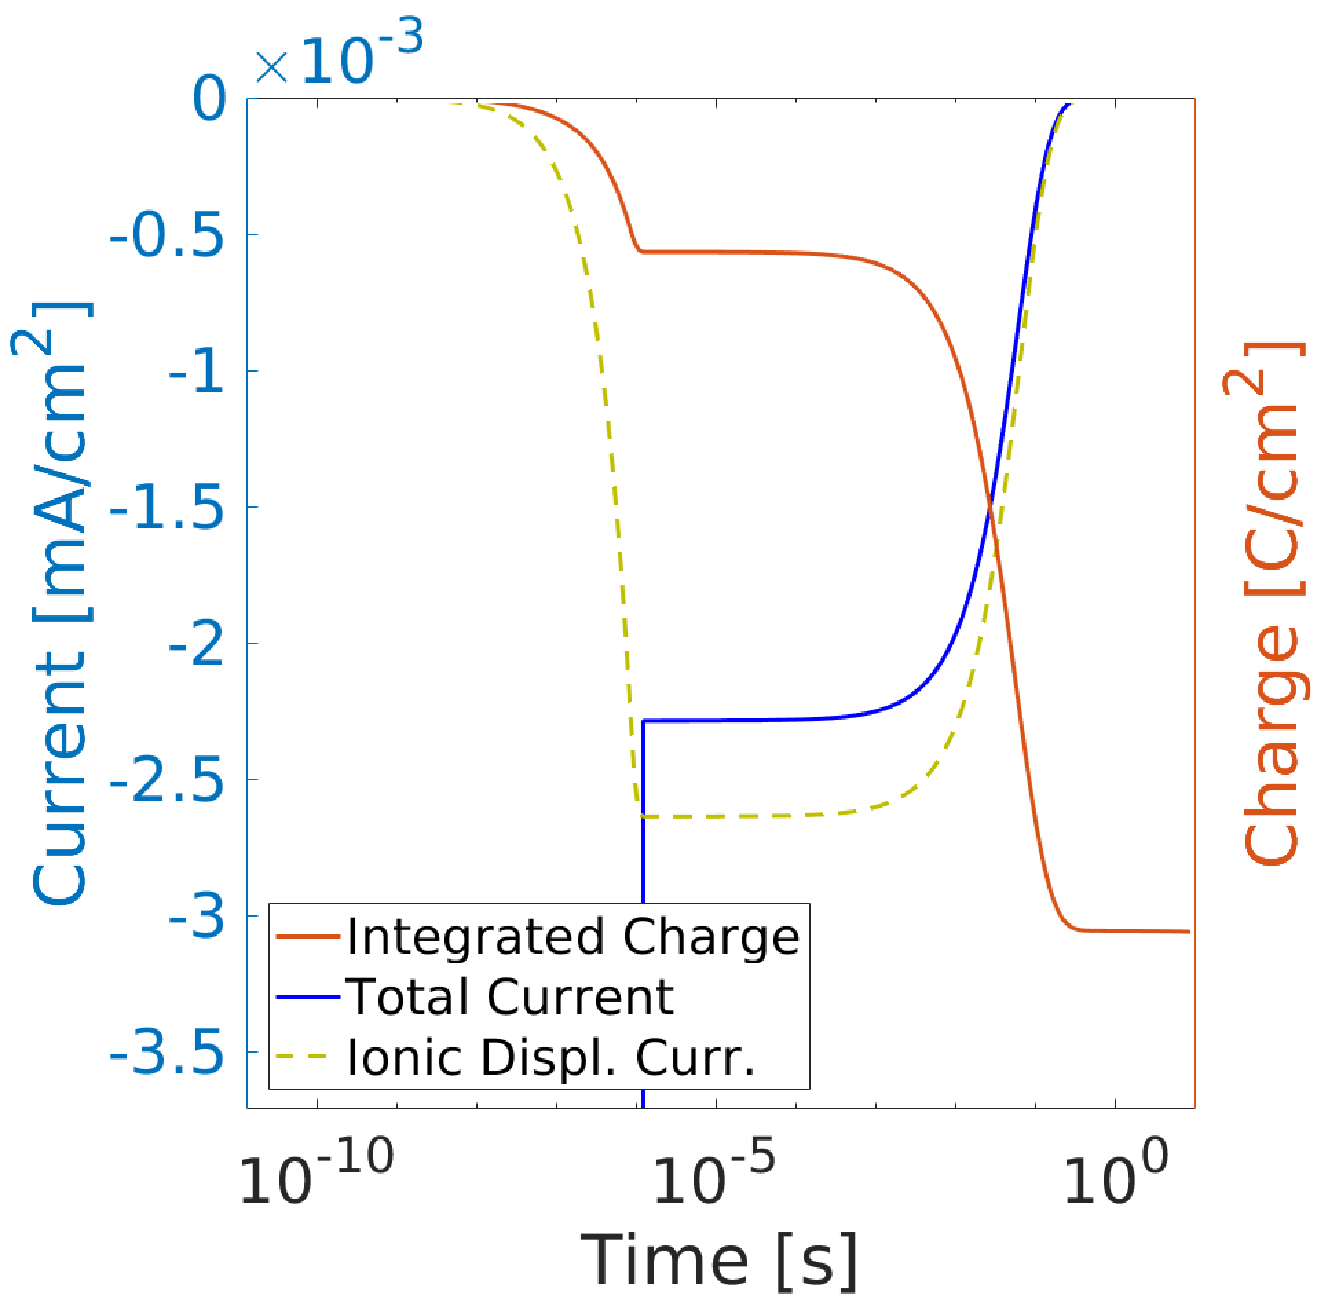
\includegraphics[width=1\textwidth]{ce_single_dd/ce_single_dd-ions_zoom.pdf}
					\subcaption{With mobile ions, magnified left axis}\label{fig:ce_single_dd-ions_zoom}
				\end{subfigure}
			}
		}
		\mycaption[Simulation of a CE without or with mobile ions.]{
			The current \textit{versus} time profile of a \acr{ce} simulated experiment is shown on the left axis just for the 1~sun illumination intensity.
			On the right axis the cumulative integration of the extracted charge.
			Clearly, the extraction is unrealistically quick as the resistance included in a real \acr{ce} experiment was not included in the simulation.
			In (\textbf{a}) the measurement of a device without mobile ions is shown, we can observe just one current peak contributing to the integrated charge; in (\textbf{b}) the presence of the mobile ions introduces a long-times contribution to the extracted charge, the current causing this is very weak and long lasting, it can be better observed in the magnification in (\textbf{c}).}\label{fig:ce_single_dd}
	\end{figure}

	%\paragraph{Interpretation of the single measurement}
	%From some preliminary and unpublished simulations of \acr{ce} show that a short living exponential decay can be accounted for free charges and a long living and weak exponential decay is caused by a displacement current due to ionic profile updating to the new voltage. The slow decay is not usually measured and seldom reported\cite{ORegan2015b}.

	\paragraph{Procedure}
	The device is kept under 1~sun equivalent illumination by a white \gls{led} at open circuit conditions until stabilization is reached.
	1~sun equivalent illumination is defined as the illumination at which the a silicon photodiode gives the same \gls{jsc} as under calibrated 1~sun from the solar simulator.
	The \gls{led}-solar spectral mismatch affects slightly the measurement, but in no case a \gls{pce} is reported from any \gls{led}-illuminated experiment.
	After stabilization the illumination is switched off and, at the exactly same moment, the device is short circuited through a small and known resistance of \SI{50}{\ohm}.
	This is repeated decreasing the light intensity from 1~sun down to dark (in dark no signal should be observed, indeed some residual charge can usually be seen, the reason of this could be ionic profile updating or an insufficient darkness) and a single decay is measured for each illumination point, over approximatively 30 illumination points.
	The equipment includes two transistors (in a home made circuit by Dr.\ Javier Pérez Hernández) connected to a pulse generator providing a square pulse long at least as the measurement window.
	From my experience, I recommend to use a short dark period in order to save time for the following stabilization step.
	The measurement is carried out with an oscilloscope in parallel to the known small resistance.
	In the first microseconds, most of the free charge flows through the resistor generating a voltage drop across it which is measured by the oscilloscope.
	This potential drop can be converted to current using the Ohm's law, which, integrated over time, gives the amount of extracted charge.

	\paragraph{Noise sources} \label{ce_noise}
	The lack of complete stabilization of the device before the extraction of charge can introduce both an error in the measured \gls{voc} and in the extracted charge.
	Regarding the \gls{voc}, in perovskite solar cells it not only depends on the illumination intensity, but it also evolves slowly until the stabilization at the steady state value, so a well defined stabilization procedure is key for achieving reproducibility in \acr{ce} experiments.
	Regarding the extracted charge, the ionic profile can influence the amount of accumulated charge, as shown for two extreme cases of presence/absence of ionic charges in \cref{fig:ce_full_dd}, so a reproducible procedure for device stabilization will also improve the reproducibility of the integrated current amount.
	Additionally, the measurement equipment introduces some electronic noise whose effect can be mitigated through data post-processing.

	\paragraph{Reduction of instrumental noise}\label{r_ce_noise}
	Most of the observed short-time noise (\SI{< 5E-7}{\s}) observable in \cref{fig:ce_noise-normal} is related to the opening and closing of the transistor switches included in the home-made circuit.
	The characteristic frequencies of the observed noise are not small compared to the measurement window, so its time-integral does not necessarily sum to zero.
	In order to reduce its impact, various approaches have been tested and here described.
	The noise can be ignored in some cases, but it's a problem if the charge \textit{versus} light bias (\gls{voc} generated at a given illumination intensity) profile, reported on the right hand column of \cref{fig:ce_noise}, has to be studied in detail, as in \cref{ch:tae}.
	In the mentioned case, just the exponential part of its linear plus exponential behaviour, reported in the bottom of each right hand figure, was of interest and it is evident that the employed noise-reduction method influences it heavily.

	\paragraph{Reduction of instrumental noise -- subtraction of dark noise}
	Annoyingly, the noise profile is characteristic of the cell and of the circuitry, so a simple average over many decays does not help in cancelling it.
	Based on this consideration, I tried to subtract a pure noise profile as obtained from a dark measurement (without any light bias).
	The operation was made more difficult by the slight variations of the noise profile with the light bias.
	A data-to-morphed-noise fit was implemented where the $f(t)$ noise profile was transformed with: $t'= u_1 + u_2 \cdot t + u_3 \cdot t^2$ and $f'(t') = u_4 \cdot f(t') + u_5 \cdot t' \cdot f(t') + u_6 \cdot e^{-t'/u_7}$ where $u_{1-7}$ are constrained fit variables.
	Then $u_6$ was set to zero and the resulting profile was subtracted from the data and the result integrated.
	As can be seen in \cref{fig:ce_noise-subtractDark}, this technique is working for most of the cases but it can fail if the noise profile changes in a more complex fashion.


	\paragraph{Reduction of instrumental noise -- integration of a fitting} Finally the decays were fitted with a bi-exponential formula (sum of two exponential) or, if the bi-exponential fitting was not converging, by a simple exponential and the integral of this fit was used.
	In both cases a robust fitting routine was employed \cite{Maechler2018}.

	\begin{figure}
		\makebox[\textwidth][c]{
			\parbox{1.1\textwidth}{
				\centering
				%				\begin{subfigure}[t]{0.55\textwidth}
				%					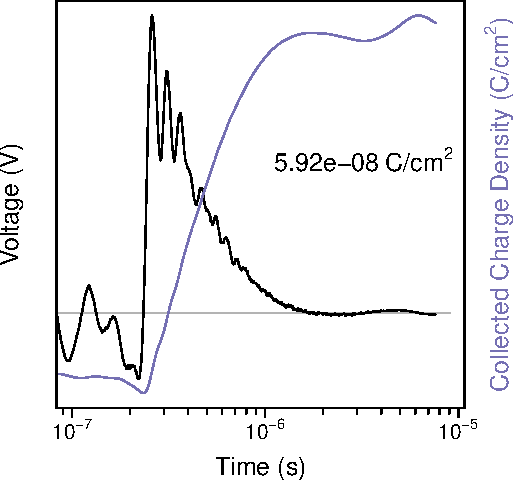
\includegraphics[width=1\textwidth]{{ce_noise/normal-CE_ig104-1566-4_Voc_0.911mV-crop}.pdf}
				%					\subcaption{Direct integration}\label{fig:ce_noise-normal}
				%				\end{subfigure}
				%				\qquad
				%				\begin{subfigure}[t]{0.35\textwidth}
				%					%\includegraphics[width=1\textwidth]{ce_noise/normal-spiro_vs_TAEs-TPVCEs_nogeom-crop.pdf}
				%					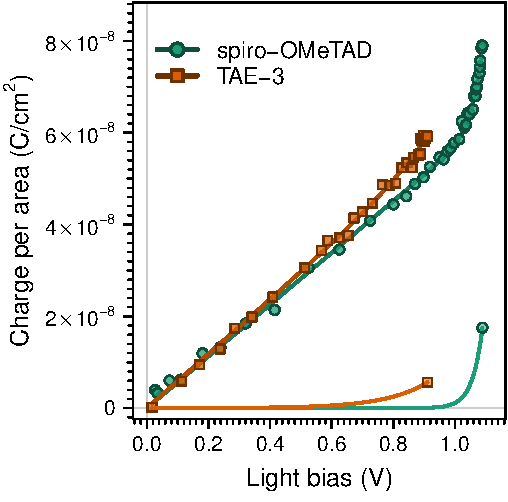
\includegraphics[width=1\textwidth]{ce_noise/normal-spiro_vs_TAEs-CEs-crop.pdf}
				%					\subcaption{Results from direct integration}\label{fig:ce_noise-normal_ce}
				%				\end{subfigure}
				%				\bigskip
				%				
				%				\begin{subfigure}[t]{0.55\textwidth}
				%					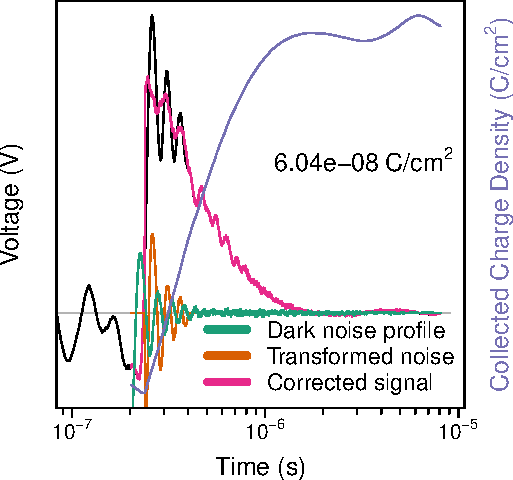
\includegraphics[width=1\textwidth]{{ce_noise/subtractDark-CE_ig104-1566-4_Voc_0.911mV-crop}.pdf}
				%					\subcaption{Subtraction of noise}\label{fig:ce_noise-subtractDark}
				%				\end{subfigure}
				%				\qquad
				%				\begin{subfigure}[t]{0.35\textwidth}
				%					%\includegraphics[width=1\textwidth]{ce_noise/subtractDark-spiro_vs_TAEs-TPVCEs_nogeom-crop.pdf}
				%					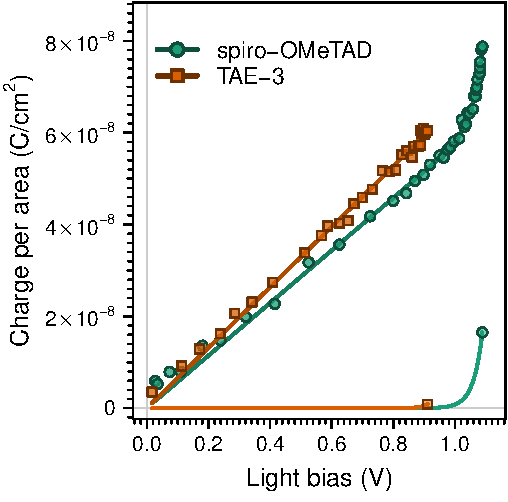
\includegraphics[width=1\textwidth]{ce_noise/subtractDark-spiro_vs_TAEs-CEs-crop.pdf}
				%					\subcaption{Results from subtraction of noise}\label{fig:ce_noise-subtractDark_ce}
				%				\end{subfigure}
				%				\bigskip
				%				
				%				\begin{subfigure}[t]{0.55\textwidth}
				%					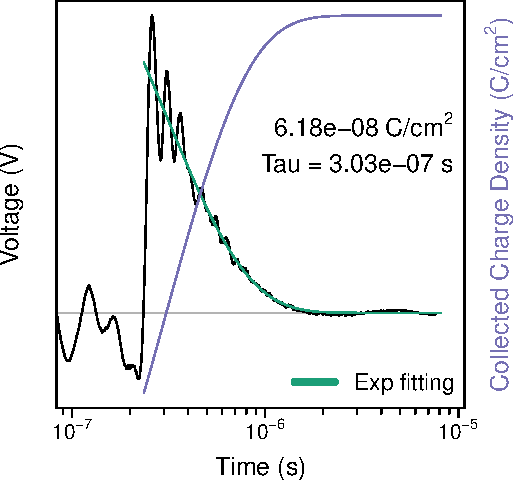
\includegraphics[width=1\textwidth]{{ce_noise/integrateExp-CE_ig104-1566-4_Voc_0.911mV-crop}.pdf}
				%					\subcaption{Integration of fitting}\label{fig:ce_noise-integrateExp}
				%				\end{subfigure}
				%				\qquad
				%				\begin{subfigure}[t]{0.35\textwidth}
				%					%\includegraphics[width=1\textwidth]{ce_noise/integrateExp-spiro_vs_TAEs-TPVCEs_nogeom-crop.pdf}
				%					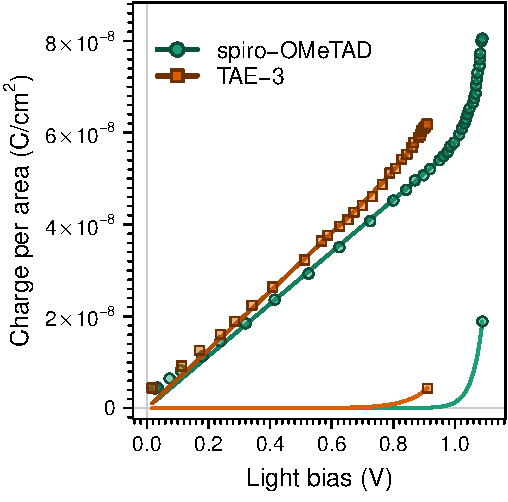
\includegraphics[width=1\textwidth]{ce_noise/integrateExp-spiro_vs_TAEs-CEs-crop.pdf}
				%					\subcaption{Results from integration of fitting}\label{fig:ce_noise-integrateExp_ce}
				%				\end{subfigure}
				\begin{subfigure}[t]{1\textwidth}
					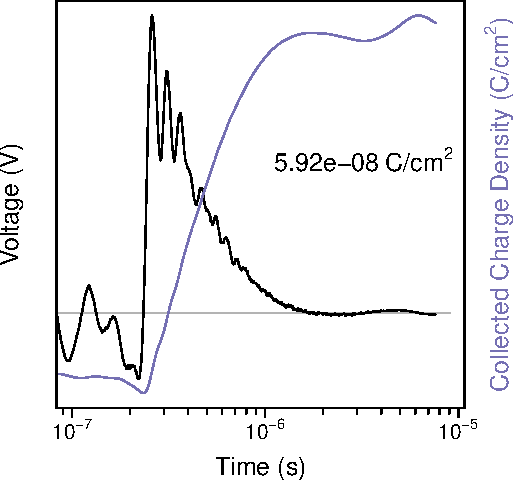
\includegraphics[width=0.45\textwidth]{{ce_noise/normal-CE_ig104-1566-4_Voc_0.911mV-crop}.pdf}
					\qquad
					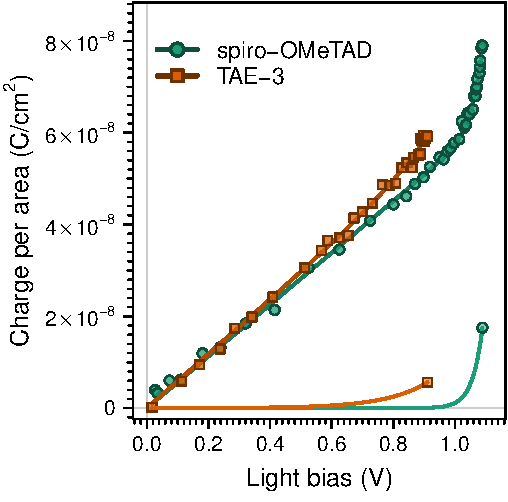
\includegraphics[width=0.35\textwidth]{ce_noise/normal-spiro_vs_TAEs-CEs-crop.pdf}
					\subcaption{Direct integration of raw data}\label{fig:ce_noise-normal}
				\end{subfigure}
				\bigskip

				\begin{subfigure}[t]{1\textwidth}
					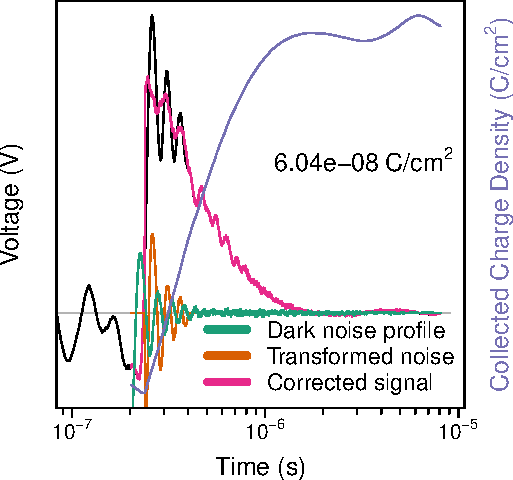
\includegraphics[width=0.45\textwidth]{{ce_noise/subtractDark-CE_ig104-1566-4_Voc_0.911mV-crop}.pdf}
					\qquad
					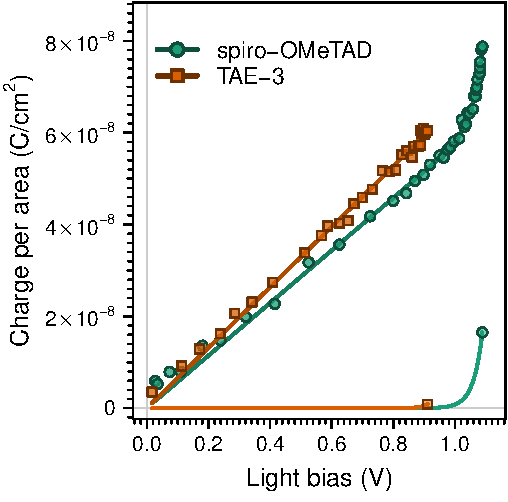
\includegraphics[width=0.35\textwidth]{ce_noise/subtractDark-spiro_vs_TAEs-CEs-crop.pdf}
					\subcaption{Subtraction of morphed noise profile}\label{fig:ce_noise-subtractDark}
				\end{subfigure}
				\bigskip

				\begin{subfigure}[t]{1\textwidth}
					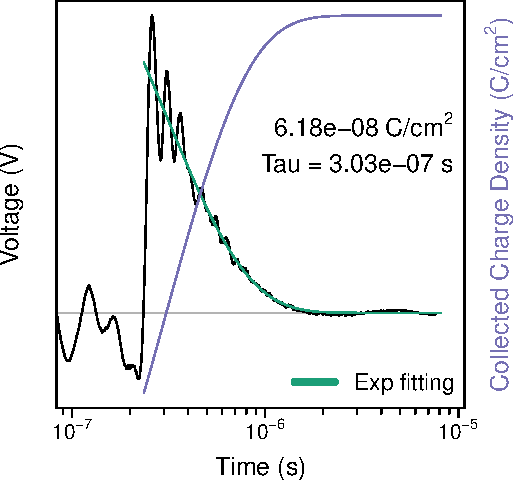
\includegraphics[width=0.45\textwidth]{{ce_noise/integrateExp-CE_ig104-1566-4_Voc_0.911mV-crop}.pdf}
					\qquad
					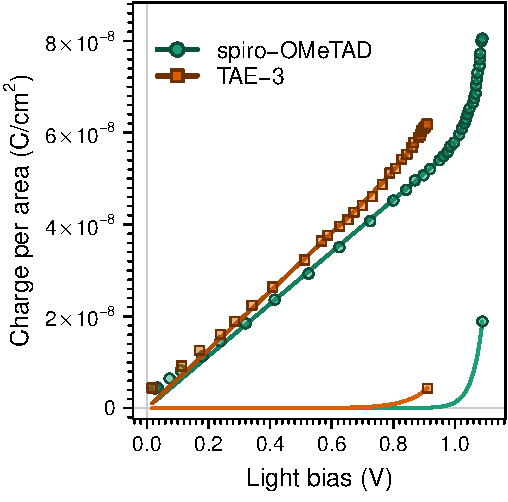
\includegraphics[width=0.35\textwidth]{ce_noise/integrateExp-spiro_vs_TAEs-CEs-crop.pdf}
					\subcaption{Integration of an exponential fitting}\label{fig:ce_noise-integrateExp}
				\end{subfigure}
			}
		}
		\mycaption[Strategies for reducing the instrumental noise in a single \gls{ce} integration.]{
			On the left, a single \gls{ce} decay from a \gls{fto}\-/\dTiOtwo\-/\mpTiOtwo\-/\acr{csfamapbibr}\-/\tae3\-/Au is integrated without noise reduction in (\textbf{a}), adapting the noise profile from the dark measurement and subtracting it in (\textbf{b}), or fitting the decay and integrating the fit in (\textbf{c}).
			On the right, the charge \textit{versus} voltage trends obtained applying the respective noise reduction methods.}\label{fig:ce_noise}
	\end{figure}



	\subsection{Interpretation of Charge Extraction}\label{interpretation_ce}

		\paragraph{Charge extracted}
		The integrated charge is assumed to include the excess free charges in the valence and conduction bands.
		With \emph{excess} we refer to the difference between the charge concentration in the conditions of interest and the stabilized dark condition.
		For a non perfectly crystalline material, localized shallow traps constituted by the tails of the valence and conduction bands density of states inside of the so-called mobility gap \cite{Pieters2009} are not negligible and should also contribute to the extracted charge amount\cite{Kirchartz2012}.
		On the contrary, charges trapped in deep traps contributing to SRH trap mediated recombination, with energies far from the band edges, should not be possible to extract in a \acr{ce} experiment.

		\paragraph{\Acr{ce} time constant}
		The free charges extraction time is related to the RC time of the \SI{50}{\ohm} resistor and the capacitance of the solar cell device.
		We can see in \cref{fig:chargeExtraction_RCtime} a weak covariance (Pearson correlation coefficient of 0.3) between the RC time obtained extrapolating the dark capacitance from \acr{dc} (which is the geometric capacitance) and the extraction time (as obtained by an exponential fitting to a single \acr{ce} current decay) at low light intensity (enough for having a signal but far from 1~sun light intensity).
		At higher light intensities, the correlation is weaker as the capacitance is less defined as the cell is in a transition between illuminated (high capacitance) and dark (low capacitance) status.
		Anyway, the extraction time does not change much between low light intensity and 1~sun with an increase from \SIrange{1.1}{2.4}{times} (first and third quartile).
		More discussion on this topic can be found on \authoryear{Montcada2018}.

		\begin{SCfigure}%[!hbtp]%
			\centering
			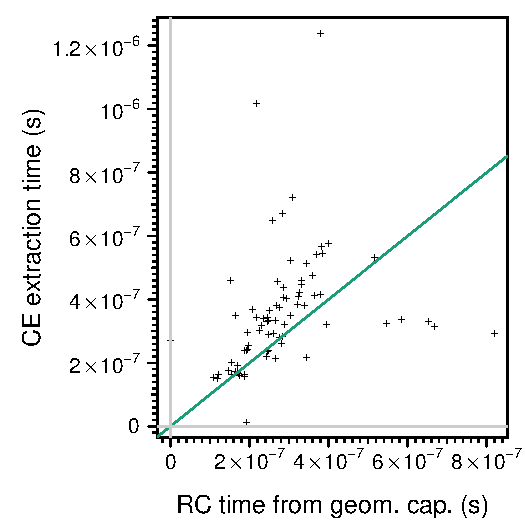
\includegraphics[width=0.45\textwidth]{chargeExtraction_RCtime/CEaBitOfSunExpTime_vs_RCdarkTime.pdf}
			\mycaption[Charge extraction time is related to a RC time.]{
				Covariance of \acr{ce} extraction time at low light intensity \textit{versus} the expected time from geometric capacitance (as obtained from dark \acr{dc}).
				Each point is a different device for a total of 78 devices, many different structures studied during my PhD are represented.
				The green line indicates the 1 to 1 relationship.}\label{fig:chargeExtraction_RCtime}
		\end{SCfigure}

		\paragraph{\Acr{ce} time constant and \acr{tpv} time constant -- Corrections}
		During this time, and depending on its location in the device stack, some free charge can recombine.
		One could argue that a \acr{ce} measurement is valid only if the extraction is faster than the recombination time as measured via \acr{tpv} \cite{Ryan2017a} or that the extracted charge should be corrected considering the recombination \cite{Credgington2011,Credgington2014}.
		Considering the charges accumulated in the depletion layers in the selective contacts, these will flow to the electrodes without crossing the perovskite/selective contacts interfaces, where has been reported that most of the recombination occurs \cite{Barnea-Nehoshtan2014,Stolterfoht2018a,Stolterfoht2018}.
		So this part of the extracted charge, distinguishable as the linear part of the charge \textit{versus} voltage plot, as represented on the right column of \cref{fig:ce_noise} should not be corrected.
		Instead, regarding the charge accumulating in the perovskite layer, which we assume can be assigned to a chemical capacitance and can be recognized as the exponential part on the right column of \cref{fig:ce_noise}, it may be that a correction \cite{Shuttle2008a,Shuttle2008b} is needed, but this has not be done in this thesis.

		\paragraph{\Acr{ce} time constant and \acr{tpv} time constant -- Correlation?}
		Some covariance (Pearson correlation coefficient of~0.4) can be observed in \cref{fig:ce_1sun_time_vs_tpv_1sun_time} between the \acr{ce} and the \acr{tpv} time constants at 1 sun illumination.
		This is unexpected and weird as the two times change with very different trends with light bias (when changing the preconditioning light intensity, \gls{ce} extraction time changes just slightly while \gls{tpv} decay time varies over various orders of magnitude).
		In case a stronger proof of correlation is found, this could indicate that both processes, even if not of the same nature, are limited by the same diffusion process, for example the migration of free charges from all the absorber to the absorber/contacts interfaces.

		\begin{SCfigure}%[!hbtp]%
			\centering
			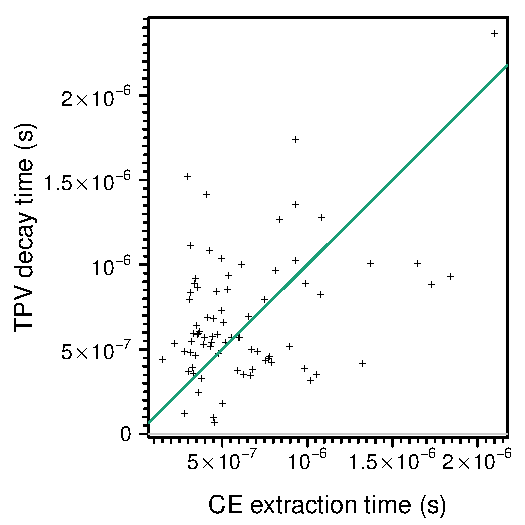
\includegraphics[width=0.45\textwidth]{ce_1sun_time_vs_tpv_1sun_time/ce_1sun_time_vs_tpv_1sun_time.pdf}
			\mycaption[Comparison between \gls{ce} and \gls{tpv} exponential decay times.]{
				Covariance of \acr{ce} extraction time at 1~sun light intensity \textit{versus} the \gls{tpv} mono-exponential decay time at 1~sun light intensity.
				Each point is a different device for a total of 79 devices, including many different structures.
				The green line indicates the 1 to 1 relationship.}\label{fig:ce_1sun_time_vs_tpv_1sun_time}
		\end{SCfigure}

		\paragraph{Charge \textit{versus} light bias trend - Exponential part in \gls{osc}}
		In \gls{osc} literature the charge \textit{versus} light bias voltage trend is described simply as the exponential shape which describes a Maxwell--Boltzmann distribution for a two levels scenario.
		For a common solar cell working conditions, the Maxwell--Boltzmann classical particles approximation should be valid as the distance between Fermi level energy and the band edges is expected to be always much bigger than $k_BT$.
		This could be false for high applied voltages, where Fermi--Dirac distribution for fermions should be used.
		$$n_{CE} = n_{DOS} \exp\left(\frac{qV - E_g}{k_BT}\right) = n_{0,CE} \exp\left(\frac{qV}{k_BT}\right)$$
		In some cases an ideality factor $m$ is introduced \cite{Kirchartz2012}, which can help to account for the shape of the density of states of the conduction band, so the expression can be found as:
		$$n_{CE} = n_{0,CE} \exp\left(\frac{qV}{mk_BT}\right)$$
		%This ideality factor $m$ is ignored in this thesis as the noise in both independent and dependent variables, even if limited with care as explained in \cpageref{ce_noise}, hinders the inclusion of an additional fitting parameter.

		\paragraph{Charge \textit{versus} light bias trend - Linear part}
		With the introduction of selective contacts, a linear contribution starts to grow in importance summing up to the exponential part.
		This linear trend accounts for the accumulation in the selective contacts and electrodes, in a parallel plate capacitor fashion \cite{Gelmetti2017,Ryan2017a,Wheeler2017,Du2018}: $Q = C_g \cdot V = \frac{\epsilon_0 \epsilon_r A}{d} \cdot V$ where $C_g$ is the geometric capacitance, $A$ is the active area, and $d$ is the thickness of the dielectric.
		More exactly, $d$ is the distance between the regions where the opposed charges are getting accumulated, which is the space charge layers (usually depletion layers) in the electrodes.
		So this value can be somewhat wider than just the distance separating the two electrodes interfaces.
		By consequence, $\epsilon_r$ should be considered as a thickness-weighted mean of the $\epsilon_r$ of each material between the two accumulation zones.
		The complete equation becomes:
		\begin{equation}\label{eq:ce_full}
			n_{CE} = C_g \cdot V + u_1 \cdot \left[\exp\left(\frac{qV}{mk_BT}\right) - 1\right]
		\end{equation}
		where the $-1$ was introduced for forcing the curve to cross the origin, as in steady state dark conditions both the \gls{voc} and the extracted charge are defined as zero.

		\paragraph{Charge \textit{versus} light bias trend - Linear part with mobile ions}
		The presence of mobile ions in perovskite materials which can accumulate at the perovskite/contacts interfaces, adds an additional capacitance $C_{ion}$, which sums up to the geometric capacitance $C_g$ increasing the weight of the linear component, as we showed in \authoryear{Moia2019}.
		Nevertheless, as pointed out in \cpageref{ce_limitations_perovskite}, the \acr{ce} measurements are never carried on for long enough to include the ionic migration, and so also the ionic accumulation capacitance gets ignored in our experiments.
		This can be visualized with the simulation reported in \cref{fig:ce_full_dd} where the long timescale (where the current is monitored until complete stabilization) and the short timescale (few tens of microseconds) \acr{ce} experiment are compared.
		The difference between the short and long timescale extracted charges is the linear contribution by the ionic capacitance discharge, observable as electronic current thanks to the relative displacement current.
		A simulation with frozen ions (the ionic profile was stabilized at open circuit and frozen during the \acr{ce} experiment) was also performed but not reported, the extracted charge is identical to the reported short timescale extraction simulation.

		\begin{figure}%[!hbtp]%
			\makebox[\textwidth][c]{
				\parbox{1.1\textwidth}{
					\centering
					\includegraphics[width=0.9\textwidth]{ce_full_dd/ce_full_dd-crop.pdf}
					\mycaption[Simulation of a complete CE experiment: charge \textit{versus} light bias with or without mobile ions.]{
						A simulation for a homo-junction device up to 1000~sun illumination (rightmost point of each set) is reported, with three points for decade.
						For each set of points, the bigger size one indicates the 1~sun pre-illumination.
						The green crosses simulates the experimentally utilised conditions: the charge gets integrated over few microseconds, while the mobile ions didn't have enough time to start migrating.
						The orange pluses considers the charge integrated until the device stabilization, over various seconds, including also the ionic displacement current.
						The purple circles simulates a mobile-ions free device.
						The solid lines represents the linear plus exponential fit crossing (0,0) obtained with the equation $n = C_g V + u_1 \{\exp[q V / (mK_BT)] - 1\}$ where $C_g$, $P_1$, and $m$ are free fitting parameters.}\label{fig:ce_full_dd}
				}
			}
		\end{figure}

		\paragraph{Charge \textit{versus} light bias trend - Exponential part with or without mobile ions}
		As can be seen in \cref{fig:ce_full_dd}, when a device with no mobile ions is simulated longer extraction time doesn't result in more charge, as expected due to the suppression of the ionic contribution.
		The simulated geometric capacitance is similar to the one obtained from short time extraction with mobile ions but the exponential part is considerably different.
		This is caused by the very different free charge accumulation profile: the presence of an un-shielded electric field in the absorber layer causes the free carriers to accumulate close to the respective selective layer, in other words it keeps the charges away from the respective recombination centres (\textit{e.g.}\ perovskite/\gls{htm} for electrons).
		This allows the simulated ions-free device to store more charge at the same illumination intensity.

		\FloatBarrier
\section{Transient PhotoVoltage (TPV)}
	\epigraph{\textit{"Imma firin mah lazor\\pewpew pewpewpew"}}

	\paragraph{Concept} While a complete device is kept open circuit under constant illumination, a small extra illumination is added via a short laser pulse.
	The \gls{voc}, originally at its steady state value, will be perturbed due to the greater generation rate during the laser pulse.
	From the \gls{voc} \textit{versus} illumination relation for photodiodes reported in \cref{eq:voc_vs_phi} follows that the \gls{voc}, at this new higher illumination, increases (this is not always the case, as for non-stabilized perovskite solar cells \cite{Calado2016}).
	After the short pulse the \gls{voc} will slowly go back to the steady state value relative to the constant illumination.
	The dynamics of this \gls{voc} relaxation back to the steady state value is the focus of Transient PhotoVoltage experiments \cite{ORegan2004,ORegan2005,ORegan2006} (also known as PhotoVoltage Decay experiments).

	\paragraph{Procedure} The device is kept under 1~sun illumination by a white \gls{led} ring at open circuit until stabilization is reached.
	1~sun equivalent illumination is defined as the illumination at which the a silicon photodiode gives the same \gls{jsc} as under calibrated 1~sun from the solar simulator.
	Then an additional illumination pulse is provided by a nitrogen laser.
	The pulse duration (\SI{\approx 1.5}{\ns}) is shorter than the oscilloscope resolution we usually employ, so we assume that the measurement happens when the pulse is already over.
	In the literature, this is not always the case as other research groups use a \gls{led} diode for the pulsed illumination \cite{Calado2016}.
	Usually a wavelength of \SI{650}{\nm} is selected using a Rhodamine B solution\cite{RadiantDyesLaser}, this wavelength illuminates in depth the perovskite layer (in contrast to a blue light where the illumination would be absorbed within the first hundreds of nanometres of the material \cite{Bi2016}).
	During all the process, the device is connected to an oscilloscope, registering the open circuit voltage profile (the \SI{1}{\Mohm} resistance of the oscilloscope is a good approximation of open circuit).
	%An auxiliary output from the square wave pulse generator used for the pulse is used for the trigger of the oscilloscope.
	The voltage profile gets averaged over a few tens of pulses in order to increase the signal to noise ratio.
	Then the background light intensity is slightly decreased and, after the stabilization to the new steady state, the new  \gls{voc} is registered and more transients are registered.
	This process is repeated over a few tens of light illuminations from 1~sun down to dark.
	%For each illumination intensity, the reported decay is the result of averaging around 30~transients. This manages to reduce the noise.

	\paragraph{Small perturbations regime}\label{tpv_perturbation}
	The intensity of the laser pulse is attenuated using a variable neutral density filter (a partially reflecting wheel with different positions for different transmittivities) so that the voltage perturbation caused by the light pulse does not exceed \SI{10}{\mV} with 1~sun background illumination intensity.
	We consider this a "small-enough" perturbation with regards to the measured \gls{voc} (see \cpageref{perturbation} for a definition of small perturbation).
	For example, comparing the excess charge in a \gls{fto}\-/\dTiOtwo\-/\acr{csfamapbibr}\-/\spiro\-/Au solar cell at \gls{voc} and at \gls{voc}~+~\SI{10}{\mV} which can be obtained from the data in \cref{fig:ce_noise-integrateExp} fitted with \cref{eq:ce_full} we can obtain respectively a value of \SI{8.2E-8}{} and \SI{8.9E-8}{\coulomb\per\square\cm}.
	Even if we're not considering the dark charge concentration (not measurable in a \acr{ce} experiment), the smallness of the charge perturbation is arguable.
	Still, we're limited to \SI{> 3}{\mV} perturbations due to the strong noise observed in this transient measurement.
	Clearly, the pulse intensity which could be considered a "small-enough" perturbation at high background illumination is not small any more at lower illumination and definitively cannot be small at dark background conditions.
	We could regulate the pulse intensity depending on the background light intensity, to ensure its smallness, but we \emph{do not} do this in order to be able to use the \acr{tpv} data for calculating \acr{dc}, as explained in \cpageref{dc_perturbation}.
	This does not usually affect the parameter extraction from \acr{tpv} as just the high illumination intensity points are considered, in order to study the device close to its expected working conditions.
	%`Anyway quite all the information from the \acr{tpv} is obtained from the high background illumination intensity measurements.AAAAAAAAAAAAAAAAAAAAAAA



	\paragraph{Voltage and charge concentration relationship} As we assume to be in the small perturbation regime, we can study the \cref{eq:ce_full} up to the first term of its series expansion:
	\begin{dmath*}
		n(V_0 + \Delta V) \approx n(V_0) + \Delta V \cdot \left.\frac{\partial n}{\partial V}\right\rvert_{V=V_0} = n(V_0) + \Delta V \cdot \left(C_g + \frac{u_1q}{mk_BT}\exp\left(\frac{qV_0}{mk_BT}\right)\right)
	\end{dmath*}
	Assigning the last addend to $\Delta n$ we can see that the charge amount variation not only is linear with $\Delta V$ (as we're in the small perturbation regime), but it also depends on the steady state voltage $V_0$.
	This relation is studied in the differential capacitance (\acr{dc}) experiment, described further in this chapter.

	\paragraph{Voltage re-equilibration dynamics}
	For what concerns a \acr{tpv} experiment, we're just interested in the analysis of the time needed for re-equilibration to steady state conditions.
	As aforementioned, the relation between $\Delta V$ and $\Delta n$ in small perturbation regime is linear, so the lifetime extracted from a $\Delta V$ decay will have the same lifetime of the underlying $\Delta n$, which is the interesting quantity when speaking of recombination.
	This means that we can observe the variations in voltage for having a correct kinetic description of the charge amount variation.
	At steady state conditions, the time derivative of the amount of charge is zero $\partial n_0 / \partial t = g(\phi) - U(n_0) = 0$ where $g$ is the generation and $U$ is the recombination.
	Considering the situation after the end of the light pulse, so while $g$ is constant but $n$ has been increased by $\Delta n$, and using a simplified expression for the recombination including just two contributions with reaction order 1 and 2 we can write:
	\begin{dmath*}
		\frac{\partial (n_0 + \Delta n)}{\partial t} = g - k_1(n_0 + \Delta n) - k_2(n_0 + \Delta n)^2 = (g - k_1 n_0 - k_2 n_0^2) - (k_1 \Delta n + 2 k_2 n_0 \Delta n) - (k_2 \Delta n ^2) \approx - (k_1 + 2 k_2 n_0 ) \Delta n
	\end{dmath*}
	where the zeroth order term is the steady state value, so it's zero, and the second order order term can be neglected (if $\Delta n \ll n_0$ then $k_2 \Delta n^2 \ll k_2 n_0 \Delta n$).
	So the rate equation is a simple pseudo-first order reaction, and the kinetic behaviour follows an exponential description like:
	\begin{equation}\label{eq:tpv_monoexp}
		n (t) = n_0 + \Delta n_0 \cdot e^{-(k_1 + 2 k_2 n_0) t} = n_0 + \Delta n_0 \cdot e^{-k_{pfo} t}
	\end{equation}

	\paragraph{From pseudo-first order rate constant to rate constant}
	Let's consider a simple case where just a first order or a second order recombination is present.
	From the \cref{eq:tpv_monoexp} it is clear that for the first case it is easy to obtain $k_1$ as it is equal to $k_{pfo}$.
	But for the second case, to obtain $k_2$ is non-trivial as it is related to $k_{pfo}$ via the charge density \cite{ORegan2007}.
	Nevertheless, for practical reasons in this thesis $k_{pfo}$ is always considered, unless explicitly specified.
	Comparisons of $k_{pfo}$ have to be performed taking care of having similar charge densities in the devices under study if an information on underlying rate constants is sought \cite{ORegan2008}.
	For this reason, rather than comparing \acr{tpv}, we usually compare life-times referenced to charge density, as in TPV-CE experiment described in \cpageref{tpvce}.

	\paragraph{Bi-exponential decays - high background illumination}
	For some devices, rather than an exponential decay, a bi-exponential decay is observed.
	This is more frequent in bottom cathode devices including mesoporous titania layers \cite{Carnie2015,ORegan2015b}.
	With \emph{bi-exponential} decay we refer to the sum of two exponential decays with two different half-life times, like:
	$$\Delta V (t) = \Delta V_1 \cdot e^{-k_1t} + \Delta V_2 \cdot e^{-k_2t}$$
	The presence of two different recombination processes is not enough for justifying a bi-exponential decay.
	This is clear looking back to \cref{eq:tpv_monoexp}, where even treating two recombination processes with even two different reaction orders we obtained a simple exponential decay.
	What we have to remember here, is that \cref{eq:tpv_monoexp} was obtained for a zero dimensional case, like what would happen in a homogeneous chemical reaction.
	In our case, the multiple recombination centres could be spatially separated.
	If the charge concentration in the two centres is dis-entangled (is not identical at any time), the sum of two exponential decays can be expected rather than a simple exponential.
	This dis-entanglement is possible if the time needed for the free carriers to migrate from a recombination centre to the other is larger than the shorter recombination life-time.
	This can happen thanks to a large-enough distance between recombination centres together with a slow free carriers mobility.
	For example for recombination centres at different depths in the solar cell stack, like at the two perovskite/contacts interfaces.
	For laterally spaced recombination centres (\textit{e.g.} pinholes \textit{versus} well covered regions) the high mobility in the electrodes is expected to equal the quasi-Fermi levels in the two adjacent recombination centres avoiding bi-exponential decays, nevertheless reports of this phenomena have been reported \cite{Montcada2017}.

	\paragraph{Mobility limited case}
	As we just saw, the mobility is a crucial parameter for the \acr{tpv} experiment.
	As a mental exercise we can imagine a case where the mobility is so slow that the free charges take a long time to diffuse (we consider diffusion as perovskite solar cells are assumed to be field-free in the absorber layer, but the same concept would hold with charges' drift) from the generation zone (in the absorber) to the recombination centre (\textit{e.g.} at a contact/absorber interface).
	In such an extreme case the provisioning of charges to the recombination centres could become a bottleneck rather than the recombination itself.
	In this regime, a \acr{tpv} experiment would be rather insensitive to actual recombination constants and even to light intensity, giving just information about mobility.
	As the observed \acr{tpv} life-times are strongly light-intensity dependent, at least at high background illumination, we can exclude to be in this mobility-limited regime.
	This would have to be revised in case a strong illumination-dependent mobility in perovskite materials was demonstrated, as has been reported in \gls{osc} \cite{Eng2010,Shuttle2010}.

	\paragraph{Bi-exponential decays at low background illumination - large perturbations}
	While bi-exponential decays at high background illumination are often not observed, these are quite always present at lower background illumination.
	Clearly, the aforementioned explanation for bi-exponential decays at high illumination are still valid for the low illumination case.
	Additionally, when studying a decay measured at lower background light intensity, we have to remember that, at least for our group's \acr{tpv} procedure, we're out of the small perturbation regime and this could justify non-exponential decays in various ways.

	\paragraph{Bi-exponential decays at low background illumination - ionic migration}
	There is another process that can be active at the very long time scale of the recombination at low free carriers density (low background illumination): ionic migration.
	What has been observed, simulating a \acr{tpv} experiment on a homojunction device with mobile ions in the absorber layer, is that ionic profile can update to the pulse-perturbed cell condition before the extra free charges recombine.
	This causes a first exponential decay of the voltage, followed by a second exponential decay due to the actual recombination of the charges generated by the laser pulse.
	So in this case, the fast component life-time is linked to the rearrangement time of the ionic profile.

	\begin{figure}
		\makebox[\textwidth][c]{
			\parbox{1.1\textwidth}{
				\centering
				\begin{subfigure}[t]{0.9\textwidth}
					\includegraphics[width=1\textwidth]{tpv_full_dd/tpv_full_dd_noions-crop.pdf}
					\subcaption{Without mobile ions}\label{fig:tpv_full_dd_noions}
				\end{subfigure}
				\bigskip

				\begin{subfigure}[t]{0.9\textwidth}
					\includegraphics[width=1\textwidth]{tpv_full_dd/tpv_full_dd_ions-crop.pdf}
					\subcaption{With mobile ions}\label{fig:tpv_full_dd_ions}
				\end{subfigure}
				\mycaption[Simulated \gls{tpv} without and with mobile ions.]{The \gls{tpv} of a homojunction solar cell is simulated, with background illumination from \SIrange{1e-10}{1}{suns} (respectively the leftmost and the rightmost points) with 3 points per decade.
					The pulse intensity was regulated in order to not exceed \SI{8}{\mV} of perturbation.
					In (\textbf{a}) a device without mobile ions is simulated, the resulting decay is a simple exponential, so the life-time of an exponential fit is reported.
					In (\textbf{b}) a device with mobile ions in the absorber layer is reported, the resulting decay is a simple exponential at high light biases but a bi-exponential at lower background illuminations, so the two life-times from a bi-exponential fitting are reported.}\label{fig:tpv_full_dd}
			}}
	\end{figure}

	\paragraph{Bi-exponential decays at low background illumination - fast life-time plateau}
	Both the fast and the slow component of bi-exponential decays hit a maximum value (plateau) at very low light intensities.
	Looking at the fast component, assigned to the rearrangement of the ionic profile, we usually observe a constant life-time.
	This points to a background light insensitive ionic rearrangement time constant, which implies a constant ionic mobility.
	This should be further studied considering the report of illumination-dependent ionic mobility by Maier's group in \authoryear{Kim2018}.

	\paragraph{Bi-exponential decays at low background illumination - slow life-time plateau}
	Regarding the slow component at very low background light intensity, as we just assigned it to the electronic recombination.
	In drift-diffusion simulations, such a plateau is not observable.
	But in the actual experiment setup, decays life-times are limited at long times by the discharge of the through the oscilloscope resistance and through the device shunt resistance, whatever is the smallest.
	This happens with an RC time of the circuit composed by the capacitance of the device (which can be obtained via a \acr{dc} experiment) and the \SI{1}{\Mohm} resistance of the oscilloscope or the internal device resistance.
	The oscilloscope resistance could be varied using an attenuating probe (usually 10X or 100X) or a high impedance amplifier.
	This limit is often observed at low light intensities as a plateau in the \acr{tpv} life-time \textit{versus} light bias graph.
	Indeed, in \authoryear{Kiermasch2018}, where a \SI{1}{\tera\ohm} input impedance amplifier is used, the plateau is observable from \SIrange{1E-1}{1}{\s}, \textit{i.e.} three orders of magnitude higher than what we observe with our \SI{1}{\Mohm} oscilloscope.
	This affirmation is corroborated by the correlation observable in \cref{fig:tpv_RCtime}.

	\begin{SCfigure}
		\centering
		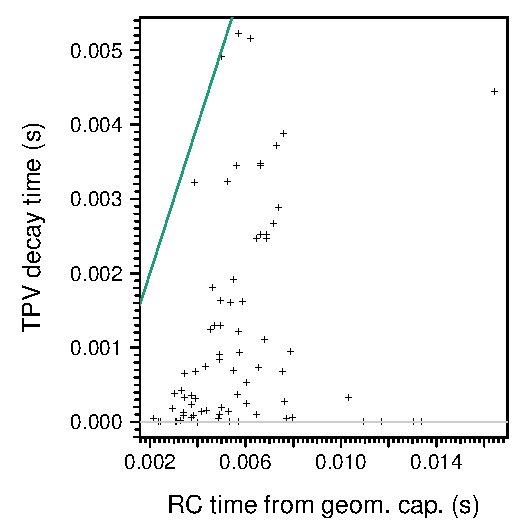
\includegraphics[width=0.45\textwidth]{tpv_RCtime/TPVdarkTime_vs_RCdarkTime.pdf}
		\mycaption[\gls{tpv} time has an upper bond due to discharge through oscilloscope.]{
			Dark \acr{tpv} time (from a robust exponential fit) \textit{versus} RC time derived from the geometric capacitance from \acr{dc} and the \SI{1}{\Mohm} of the oscilloscope.
			Each point is a different device for a total of 76 devices, including many different structures.
			The green line indicates the 1 to 1 relationship.}\label{fig:tpv_RCtime}
	\end{SCfigure}

	\paragraph{Noise treatment}\label{tpv_robust}
	Most of the observed noise (\SI{< 2E-7}{\s}) is due to the radiofrequency emitted by the spark in the nitrogen laser which gets absorbed by all the non-coaxial cables (coaxial ones don't) and from the circuitry of the samples holder acting as a receiving antenna.
	On the contrary to what happens for \acr{ce} (see \cpageref{ce_noise}), the short times noise does not follow a constant pattern, so averaging the measurement over a few repetitions (usually 30) manages to reduce the noise.

	This noise can affect the exponential or bi-exponential fitting, for this reason a robust fitting routine has been used, which gives a lower weight to outlier points.
	An example can be seen in \cref{fig:tpv_robust}.

	\begin{figure}
		\centering
		\includegraphics[width=0.9\textwidth]{{tpv_robust/TPV_ig52-68-3_0.883897_V-monoexp}.pdf}
		\mycaption[Robust and normal fitting comparison.]{In grey the fitted points, in yellow the points not considered for the fitting, the solid black line is the \gls{loess}.
			The normal non-linear least squares fitting (in green) is affected by noise, outliers and characteristics not of interest by the model.
			The non-linear robust fitting (in brown) manages to reduce the weight of these points.}\label{fig:tpv_robust}
	\end{figure}

	\paragraph{Importance of stable steady state starting point}
	The values extracted from \acr{tpv} are strongly sensible to the surface recombination and electric fields in the absorber, which in turn vary during ionic profile stabilization.
	Comparison of decay times with different stabilization times can be found in \authoryear{ORegan2015b}, while in \authoryear{Calado2016} even negative peaks are reported and explained with the presence of a residual electric field in the absorber previous to ionic profile stabilization.


\section{Transient PhotoVoltage Referenced to Charge Extraction (TPV-CE)}\label{tpvce}
	In order to obtain information on the recombination processes, it is more useful to relate the recombination life-time to the charge concentration, rather than to the light bias, as in a pure \acr{tpv} experiment.
	One way to obtain this is taking the $\tau (V)$ relation from \acr{tpv} and substituting $V$ with the inverse of $n(V)$ obtainable from \acr{ce} experiments, obtaining the $\tau (n)$ relationship.
	In \gls{osc} literature, where a simple exponential charge \textit{versus} voltage is usually observed, the full $n$ obtained by \acr{ce} is taken.
	For perovskite solar cells, the linear part of $n(V)$ related to the geometric capacitance of charges accumulating in the selective contacts cannot be ignored and a discussion on  whether to include it or not is needed.
	In this thesis
	recombination order $\Phi = \lambda + 1$ \cite{Shuttle2008d,Credgington2011}



\section{Transient PhotoCurrent (TPC)}

	\paragraph{Concept}
	This technique, applied to a solar cell at short circuit conditions, allows us to study the dependence of \gls{eqe} on the light illumination intensity \cite{ORegan2004}.
	Just the generated charge, rather than actual value of \gls{eqe} (generated charge over incident photons ratio) is obtained as the incident power is not usually measured (on the contrary to the classical \gls{eqe} experiment).

	\paragraph{Procedure}
	The device is kept under 1~sun illumination by a white \gls{led} ring at short circuited through a \SI{50}{\ohm} resistor until stabilization is reached.
	1~sun equivalent illumination is defined as the illumination at which the a silicon photodiode gives the same \gls{jsc} as under calibrated 1~sun from the solar simulator.
	Then an additional illumination pulse is provided by a nitrogen laser.

	The signal is acquired by an oscilloscope in parallel to the \SI{50}{\ohm} resistor.
	This allows us to measure a potential drop across the resistor and the related current via Ohm's law.
	Subtracting the constant current due to the background illumination and integrating the transient over time gives the charge generated by the laser pulse.

	This process is repeated at 1~sun and at dark background illumination conditions.

	For each illumination intensity, the reported decay is the result of averaging around 30~transients.
	This manages to reduce the noise.


	\paragraph{Dependency on background illumination}
	When measuring \acr{tpc} at various background illumination intensities, a constant pulse-generated charge amount can be gathered for low illuminations that starts decreasing as the background illumination exceeds \SI{1}{sun} (as reported for perovskite solar cells in figure S5 of \cite{Du2018}).
	In \gls{osc} this was assigned to primary geminate recombination, which, as seen in \cpageref{intro_geminate}, is negligible in perovskite materials.
	Other kind of recombination can affect the extracted charge, even in short circuit conditions, if the charge extraction is not sufficiently quick.
	For this reason, in case of large discrepancies between the dark and the \SI{1}{sun} background illumination measures, the dark one better describes the photo-generated free-charge.
	The influence of the different electric field on the absorption, explained in \cpageref{intro_electroabsorbance}, can be neglected as the field is screened in most of the absorber and anyway the electro absorbance phenomena should have just a small contribution.






	%	For the interpretation, see \cpageref{interpretation_tpc}; for the implementation, see \cpageref{r_tpc}.

\section{Differential Capacitance (DC)}
	In the differential capacitance experiment (also known as differential charging)
	This is a meta-measurement as it just combines the data from \acr{tpv} and \acr{tpc} without requiring any additional experiment \cite{ORegan2005,ORegan2006,Shuttle2008}, sometimes also referred to as "differential capacitance".

	As explained in \cpageref{interpretation_dc}, the electrical capacitance of a solar cell is not a constant (as in most of the commercial capacitors), indeed it depends on the applied voltage bias or light bias.
	\\

	The charge obtained with the \acr{tpc} (in case the dark and illuminated results were different, the third quartile of all \acr{tpc} measurements was used) is divided by an array of values obtained from \acr{tpv}, one for each illumination intensity.
	The needed value is the \gls{voc} increase due to the laser pulse, prior to the decay to steady state, for each illumination intensity.

	This allows us to estimate the capacitance of the solar cell device at open circuit with various illumination intensities.

	\paragraph{Small perturbations}\label{dc_perturbation}
	As mentioned in \cpageref{tpv_perturbation}, we measure \acr{tpv} ensuring to be in the small perturbation conditions for high light bias illumination.
	But the perturbations are surely large getting close to dark illumination conditions.
	This happens because we're not changing the laser pulse intensity when decreasing the background illumination.
	This way, we can measure just one \acr{tpc} for knowing the amount of generated charge, as we assume that it depends just on the laser pulse intensity.
	The measure of as many \acr{tpc} as many laser pulse intensities would be too complex with our current experimental setup.
	%	The \acr{dc} does not intrinsically need the usage of a constant pulse intensity but it needs the measurement of a \acr{tpc} for each pulse intensity.
	%The switch from \acr{tpv} to \acr{tpc} setup and back would be complex and too time demanding with the current setup.

	\paragraph{Voltage peak value from \acr{tpv}}\label{tpv_deltaV}
	%The value of the voltage increase due to the additional illumination is needed for \acr{dc} measurement.

	In our group, the $\Delta V$ value has been extracted  obtained subtracting the steady state \gls{voc} from the maximum voltage point in the measured transient.
	This is obviously heavily affected by the aforementioned noise when a short time window is used.

	The following alternatives were tested:
	\begin{itemize}
		\item The linear factor in an exponential fit was used, but it can fail if the decay does not have a simple exponential shape (often a bi-exponential, sum of two exponentials, is observed);
		\item The sum of the two linear factors in a bi-exponential fit, which could work but one have to carefully set boundary values to the fitting parameters for avoiding a fast exponential matching just some noise;
		\item The maximum value of a \gls{loess} local regression was used, but this underestimates the value, especially when the peak top are just few points (when the measurement time window is large);
		\item The average of the values registered starting from the maximum voltage point and during a specified time lapse.
	\end{itemize}

	This last option is the one currently in place.
	The average was performed over \SI{50}{ns} after the peak and this allowed us to get a reliable $\Delta V$ value.

	\paragraph{Capacitance from voltage and current increase during the pulse}
	In case a slow light pulse have to be employed, \textit{e.g.} from a \gls{led} source, the voltage peak is too strongly affected by the ongoing recombination.
	An alternative method considering the plateau current of a \acr{tpc} experiment \textit{versus} the voltage grow rate from \acr{tpv} has been reported in \authoryear{ORegan2015b}.

	\paragraph{Comparison of charge from DC and from CE}
	The \acr{dc} experiment has been demonstrated to output a very similar charge \textit{versus} light bias profile as a \acr{ce} experiment when used for \gls{dssc} \cite{ORegan2005,Barnes2013} and in \gls{osc} \cite{Shuttle2008a}.
	\Acr{dc} started to be employed in perovskite solar cells characterization due to the excessively large charge amount sometimes measured by \acr{ce} \cite{Wheeler2017,ORegan2015b}.


\section{Impedance Spectroscopy}

\section{Stark Spectroscopy (ElectroAbsorbance)}

\section{Interpretation of Kelvin Probe Force Microscopy}\label{interpretation_kpfm}

\section{Molecular Characterization}
	\subsection{Interpretation of Band Gap Values Obtained via Tauc Plot, PhotoLuminescence and Computational Simulations}\label{interpretation_bg}

		%	Otra cosa, flipé mucho con la respuesta del Vidal y me puse a intentar
		%	ver que se supone que se saca del espectro experimental y desde cual
		%	pico. Como el dijo, las simulaciones son correctas.
		%	Pero, creo que sea mi concepto (el HOMO-LUMO está bastante lejos del
		%	absorption onset, como demostrado de sus simulaciones donde el
		%	absoprtion onset, por ejemplo de TAE-1, está a 2.9 eV y el HOMO-LUMO gap
		%	está a 5.06 eV) que lo de Vidal (el pico de máxima absorción no tiene
		%	nada a que ver con el HOMO-LUMO gap, en mi opinión para nada) estaban
		%	totalmente equivocados y que habría que enviar a medir el UPS de las
		%	moléculas para sacar el HOMO-LUMO gap.
		%
		%	El concepto está explicado en el primer párrafo de esta pagina:
		%	https://chemical-quantum-images.blogspot.com/2013/06/why-is-homo-lumo-gap-not-good-guess-of.html
		%
		%	Lo que he puesto, o sea que lo hemos medido por Tauc plot, creo colaría
		%	porque todo el mundo lo mide así y está bien aceptado como método. Pero
		%	la verdad es que es valido solo para semiconductores donde los orbitales
		%	están bien deslocalizados, no como nuestra molécula en solución donde el
		%	estado es bien localizado en la molécula.

\section{Our Solar Cells Characterization Steps}

	In this section I'll describe the routinary characterization performed in Palomares group.


